%%%%%%%%%%%%%%%%%%%%%%%%%%%%%%%%%%%%%%%%%%%%%%%%%%%%%%%%%%%%%%%%%%%%%%%
% Slides for the TechCon 2022 talk "PyAnsys tools for unit testing" 
%%%%%%%%%%%%%%%%%%%%%%%%%%%%%%%%%%%%%%%%%%%%%%%%%%%%%%%%%%%%%%%%%%%%%%%
\documentclass[t]{beamer}

\usetheme{Ansys2022}

\usepackage{minted}
\usepackage{xcolor}
\usepackage{pdfpages}
\usepackage{listings}
\usepackage{tikz}
\usepackage{hyperref}

\usepackage[edges]{forest}
\hypersetup{
    colorlinks=true,
    linkcolor=blue,
    filecolor=magenta,      
    urlcolor=cyan,
}
 

\urlstyle{same}
\setbeamercolor{background canvas}{bg=}

\definecolor{bleudefrance}{rgb}{0.19, 0.55, 0.91}

%%%%%%%%%%%%%%%%%%%%%%%%%%%%%%%%%%%%%%%%%%%%%%%%%%%%%%%%%%%%%%%%%%%%%%%%%%%%%%%
\usetikzlibrary{shapes.geometric, arrows,positioning}

\tikzset{
  startstop/.style={
    rectangle, 
    rounded corners,
    minimum width=3cm,
    minimum height=0.75cm,
    align=center, 
    draw=black, 
    fill=ANSYS@Gold,
    },
  process/.style={
    rectangle, 
    minimum width=3cm, 
    minimum height=0.75cm, 
    align=center, 
    draw=black, 
    fill=ANSYS@Blue,
    text=white,
    },
  decision/.style={
    diamond, 
    aspect=4,
    minimum width=3cm, 
    minimum height=1cm,
    align=center,
    draw=black, 
    fill=ANSYS@Blue,
    text=white,
    },
  arrow/.style={thick,->,>=stealth},
  dec/.style={
    ellipse, 
    align=center, 
    draw=black, 
    fill=ANSYS@Bronze,
    },
}

\begin{document}

%%%%%%%%%%%%%%%%%%%%%%%%%%%%%%%%%%%%%%%%%%%%%%%%%%%%%%%%%%%%%%%%%%%%%%%%%%%%%%%
%% Title Slide

\title{PyAnsys tools for unit testing}
\subtitle{Applying test-driven development}
\author{Author: PyAnsys Core Team}
\date{\today}

\titleframe{}


%%%%%%%%%%%%%%%%%%%%%%%%%%%%%%%%%%%%%%%%%%%%%%%%%%%%%%%%%%%%%%%%%%%%%%%%%%%%%%%
%% Table of contents

\begin{frame}{Table of Contents}
  \tableofcontents
  \vspace{200pt}  %% force top left  
\end{frame}


%%%%%%%%%%%%%%%%%%%%%%%%%%%%%%%%%%%%%%%%%%%%%%%%%%%%%%%%%%%%%%%%%%%%%%%%%%%%%%%
\section{Introduction}
\begin{frame}
  \frametitle{Content}
  \tableofcontents[currentsection]
  \vspace{200pt}  %% force top left
\end{frame}

\begin{frame}[fragile=singleslide]
  \frametitle{Introduction}

  \begin{itemize}
  \setlength\itemsep{1em}

  \item{\textbf{What is test-driven development (TDD)?}
    \\As soon as the code base gets modified, a collection of tests get executed
    to guarantee the integrity of the new code.
  }

  \item{\textbf{What are its main advantages?}
    \\It allows to generate and modify code in a faster and robust manner.
    }

        
  \item {\textbf{pytest as the main testing framework for PyAnsys}
    \\The pytest testing framework is the reference one in the Python community.
    }

  \end{itemize}

\end{frame}

%%%%%%%%%%%%%%%%%%%%%%%%%%%%%%%%%%%%%%%%%%%%%%%%%%%%%%%%%%%%%%%%%%%%%%%%%%%%%%%
\section{An overview of pytest capabilities}

\begin{frame}
  \frametitle{Content}
  \tableofcontents[currentsection]
  \vspace{200pt}  %% force top left
\end{frame}


\subsection{Basic assertions with pytest}
\begin{frame}[fragile=singleslide]
  \frametitle{Basic assertions with pytest}

   \begin{itemize}
        \item Tests are defined using functions.
        \item Use the \textit{assert} keyword to compare current and expected results.
        \item Run your tests by executing \textit{pytest vv tests}
   \end{itemize}

   \inputminted[fontsize=\footnotesize]{python}{code/basic_assertion.py}

\end{frame}

%%%%%%%%%%%%%%%%%%%%%%%%%%%%%%%%%%%%%%%%%%%%%%%%%%%%%%%%%%%%%%%%%%%%%%%%%%%%%%%
\subsection{Floating point assertions}
\begin{frame}[fragile=singleslide]
  \frametitle{Using NumPy for floating point assetions}

   \begin{itemize}
        \item For floating point values, absolute and relative tolerances are required.
        \item NumPy provides the \textit{assert\_allclose} routine for this purpose.
   \end{itemize}


   \inputminted[fontsize=\footnotesize]{python}{code/floating_point_assertion.py}


\end{frame}

%%%%%%%%%%%%%%%%%%%%%%%%%%%%%%%%%%%%%%%%%%%%%%%%%%%%%%%%%%%%%%%%%%%%%%%%%%%%%%%
\subsection{Marking tests}
\begin{frame}[fragile=singleslide]
  \frametitle{Marking tests}

   \begin{itemize}
       \item Marking tests allows to filter and select desired tests from the test suite.
       \item Marking is performed using the \textit{pytest.mark.<name>} decorator.
       \item Select marked tests by executing \textit{pytest -m <name> -vv tests}
   \end{itemize}

   \inputminted[fontsize=\footnotesize]{python}{code/marked_test.py}

\end{frame}

%%%%%%%%%%%%%%%%%%%%%%%%%%%%%%%%%%%%%%%%%%%%%%%%%%%%%%%%%%%%%%%%%%%%%%%%%%%%%%%
\subsection{Parametrizing tests}
\begin{frame}[fragile=singleslide]
  \frametitle{Parametrizing tests}

   \begin{itemize}
           \item Parametrizing a test means running the same assert on different inputs
           \item Parametrizing allows reusing test code.
           \item Parametrizing is done by using the \textit{pytest.mark.parametrize} decorator.
   \end{itemize}

   \inputminted[fontsize=\footnotesize]{python}{code/parametrized_test.py}

\end{frame}

%%%%%%%%%%%%%%%%%%%%%%%%%%%%%%%%%%%%%%%%%%%%%%%%%%%%%%%%%%%%%%%%%%%%%%%%%%%%%%%
\subsection{A plethora of plugins}
\begin{frame}[fragile=singleslide]
  \frametitle{A plethora of plugins}

   It is possible to extend the capabilities of pytest by creating and using plugins.

   \vspace{1em}

   \begin{itemize}
       \item Pytest integrates with the \textit{unittest} module from Python STD library.
       \item Pytest integrates can test for \textit{doctests} too.
       \item Code coverage with \href{https://pypi.org/project/pytest-cov/}{https://pypi.org/project/pytest-cov/}
       \item Matplotlib testing with \href{https://pypi.org/project/pytest-mpl/}{https://pypi.org/project/pytest-mpl/}
       \item Property-based testing with see \href{https://pypi.org/project/hypothesis/}{https://pypi.org/project/hypothesis/}
   \end{itemize}

   \vspace{1em}

   % Check out the official list of plugins \href{https://docs.pytest.org/en/latest/reference/plugin_list.html}{https://docs.pytest.org/en/latest/reference/plugin_list.html}

\end{frame}

%%%%%%%%%%%%%%%%%%%%%%%%%%%%%%%%%%%%%%%%%%%%%%%%%%%%%%%%%%%%%%%%%%%%%%%%%%%%%%%
\subsection{Continuous integration and development}
\begin{frame}[fragile=singleslide]
  \frametitle{Continuous integration and development}

   \begin{itemize}
        \item The continuous integration and development (CI/CD) takes place in GitHub.
        \item It is performed using GitHub Actions and configured via YML-based files.
        \item It allows PyAnsys projects to run on multiple OS under multiple Python versions.
   \end{itemize}

  \centering
  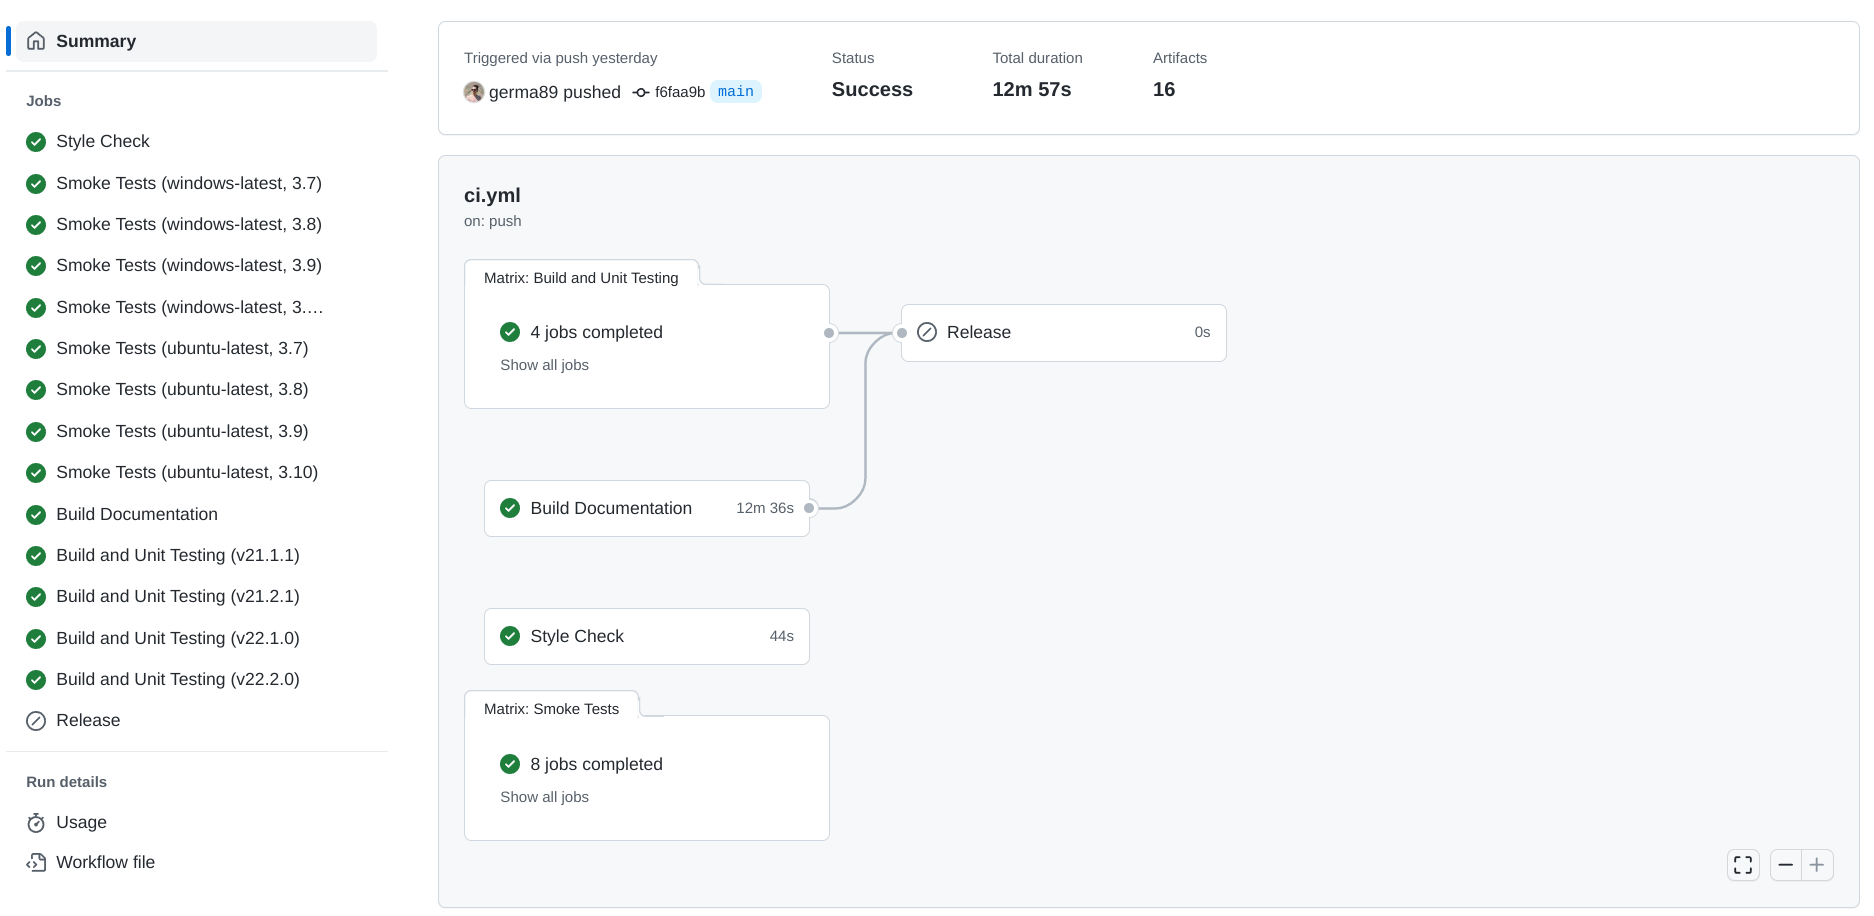
\includegraphics[height=.5\textheight]{./figures/gh_actions_pipeline.png}

\end{frame}


%%%%%%%%%%%%%%%%%%%%%%%%%%%%%%%%%%%%%%%%%%%%%%%%%%%%%%%%%%%%%%%%%%%%%%%%%%%%%%%
\subsection{Additional information on how to test your library}
\begin{frame}[fragile=singleslide]
  \frametitle{Continuous integration and development}

        For additional information on how to test your library by using pytest
        and taking advantage of CI/CD, visit the PyAnsys official developer's
        guide.

        \vspace{1em}
        \centering

        \vspace{1em}
        \textbf{How-to testing}
        \\\href{https://dev.docs.pyansys.com/how-to/testing.html}{https://dev.docs.pyansys.com/how-to/testing.html}

        \vspace{1em}
        \textbf{How-to use continuous-integration}
        \\\href{https://dev.docs.pyansys.com/how-to/continuous-integration.html}{https://dev.docs.pyansys.com/how-to/continuous-integration.html}

        \vspace{1em}
        \textbf{PyAnsys developer's guide}
        \\\href{https://dev.docs.pyansys.com/}{https://dev.docs.pyansys.com/}

\end{frame}


\lastframe{}
\end{document}
